\documentclass[letterpaper]{aamas2009}
%\usepackage{ijcai09}
\usepackage{amssymb}
%\usepackage[english]{babel}
\usepackage{latexsym}
\usepackage{amsfonts}
\usepackage{amsmath}
\usepackage{graphicx}
\usepackage{algorithmic}
\usepackage{times}
\usepackage{subfigure}
%\usepackage{natbib}
%
\def\sharedaffiliation{%
\end{tabular}
\begin{tabular}{c}}
%

\numberofauthors{3} 

\author{\alignauthor Zinovi Rabinovich\\
  \affaddr{Electronics and Computer Science}\\
  \affaddr{University of Southampton}\\
  \affaddr{Southampton, United Kingdom}\\
  \email{zr@ecs.soton.ac.uk}
\alignauthor Lachlan Dufton\\ 
  \affaddr{Cheriton School of Computer Science}\\
  \affaddr{University of Waterloo}\\
  \affaddr{Waterloo, Canada}\\
  \email{ltdufton@cs.uwaterloo.ca}
\alignauthor Kate Larson\\
  \affaddr{Cheriton School of Computer Science}\\
  \affaddr{University of Waterloo}\\
  \affaddr{Waterloo, Canada}\\
  \email{klarson@cs.uwaterloo.ca}
} 

\title{Policy  Teaching by a Modulation of the Transition Model}

\begin{document}

\maketitle

\section{Introduction}
\nocite{taylor_PhD_2008}
\nocite{taylor_stone_2009}
\nocite{fleming_hernandez-hernandez_CDC_97}
\nocite{todorov_2009_framework_sup}
\nocite{todorov_2009_framework}
\nocite{ng_russell_2000}
\nocite{zhang_parkes_2008}
\nocite{zhang_parkes_2009_ed}
\nocite{dufton_larson_2009}
\nocite{banerjee_peng_2005}

\section{Interaction Model}
Our interaction framework consists of a dynamic stochastic environment
that is influenced by two agents, a {\em learner} and a {\em
  teacher}. The learner agent receives a direct feedback from the
environment in form of a reward, that depends on the change in the
environment's state and the action chosen by the learner. We assume
that the learner is rational and, therefore, seeks an action policy
that will maximise its expected reward. To achieve this goal the
learner employs a publicly known iterative computation or a learning
algorithm, depending on environment model availability. At each
iteration of the algorithm, the chosen policy is compared with some
ideal or {\em reference} policy held by the teacher agent. The
difference between the two policies determines the cost of that stage
for the teacher agent. The teacher agent may attempt to influence the
learner's policy calculation by modifying the environment
dynamics. That is, the teacher's actions influence the way the
environment state changes in response to the learner's
actions. However, such modulation incurs additional cost to the
teacher agent. Further away the teacher pushes the environment from a
certain nominal or {\em passive} dynamics, higher the cost. In this
interaction framework, we would be interested to find a sequence of
teacher's actions that optimally balances the two costs: distance of
the learner's policy from the reference and the cost of the
environment modification.

To instantiate the above framework, we will consider for the remainder
of this paper the following Markovian environment tuple $<S,A,U,T,R>$,
where:
\begin{itemize}
\item $S$ is the state space of the environment
\item $A$ is the set of actions available to the learner
\item $U$ is the space of modifications that the teacher can apply
\item $c:S\times A\times S\rightarrow\mathbf{R}$ is the reward (or
  cost) function of the learner. $c(s',a,s)$ is the reward received by
  the learner if it has applied action $a\in A$ and the environment
  moved from state $s\in S$ to state $s'\in S$.
\item $T:S\times A\times U\rightarrow\Delta(S)$ is the transition
  function. 

$T(s'|s,a,u)$ is the probability that the
  environment state will change from $s$ to $s'$ if the learner has
  applied action $a\in A$ and the teacher chose the environment
  modification $u\in U$.

Denote $T_{u_t}(s'|s,a)=T(s'|s,a,u_t)$. We assume that there exist a null
  modification $u^*\in U$, so that $T^*=T_{u^*}$ are the nominal,
  passive dynamics of the environment.
\end{itemize}

While applying its iterative policy calculation algorithm, the learner
faces a seqence of Markov Decision Problems (MDPs)~\cite{puterman_book_94}
$<S,A,U,T_{u_t},R>$, although it is not aware of the dynamics
modulation and proceeds as if they were homogeneous. That is, at every
stage the learner seeks an action policy of the form
$\pi:S\rightarrow\Delta(A)$ that would produce the highest expected
reward if $T_{u_t}$ would persist indefinitely.\footnote{This latter
  assumption is explicit only if the learner actually has access to
  the environment model. For most standard RL algorithms this
  assumption would hold implicitly.}

Now, denote $x_t$ the internal state of the learner's policy
computation at iteration $t$, and let
$\pi_t=\pi(x_t):S\rightarrow\Delta(A)$ be the policy that corresponds
to that computation state. Also, denote $\pi^*$ the ideal reference
action policy of the learner. Then at time $t$ the teacher incurs cost
$Cost(\pi_t,u_t)$ that combines the distance between $\pi_t$ and
$\pi^*$ and between $T_{u_t}$ and $T^*$. The overall optimization
problem for the teacher is as follows, where $x_t=F(x_{t-1},u_t)$
denotes one step of the learner's compuation algorithm and $x_0$ is
known:
\begin{eqnarray*}
&\min\limits_{u_t}\sum\limits_{t=1}^{t_{max}}Cost(\pi_t,u_t)\\
&s.t.\\
&\pi_t=\pi(x_t)\\
&x_t=F(x_{t-1},u_t)
\end{eqnarray*}

Notice that the above formulation is generic with respect to the
actual algorithm employed by the learner agent. The formalism captures
both policy and value iteration algorithms, both with given and
learned environment model. It even captures the case where the learner
is capable of transfer learning. In this case learner's state $x_t$
will include structural knowledge gathered thus far from the
interaction with the environment. 

The teacher-learner interaction framework, as we have describe it
above, can also adopt various cost functions that describe how the
teacher fuses the environment modification effort and the distance of
the learner from the reference policy. However, in this work we adopt
a specific cost function based on the Kullback-Leibler divergence
rate. This enables an automic balancing between the two costs. It also
has the additional benefit to concentrate the cost dependency on those
portions of the environment dynamics that are most relevant to the
current action policy choice by the learner. In the following
subsection we describe our teacher's cost function in more detail.

\subsection{Teacher's Cost Computation}
As a measure of cost we will use Kullback-Leibler divergence rate
between two processes formed by the application of the teacher's
augmentation $u_t$ and the learner's policy $\pi_t$. More specifically,
consider the stochastic process over the state-action pairs formed by
the application of the learner's policy in the modified environment at
time $t$: \\
\centerline{$
P_t(s',a'|s,a)=T_{u_t}(s'|s,a)\pi_t(a'|s')
$}

Similarly, denote $P^*(s',a'|s,a)=T^*(s'|s,a)\pi^*(a'|s')$.

The process $P_t$ has a stationary distribution $q_t$ over $S\times
A$, so that $q_t=P_tq_t$. Notably, the stationary distribution can be
decomposed (with a slight abuse of notation) $q_t(s,a)=q_t(a|s)q_t(s)$
and then expressed by the following equations:
%% \begin{eqnarray*}
%% q_t&=&q_t(a'|s')q_t(s')=P_tq_t\\
%% &=&\sum\limits_{s,a}T_{u_t}(s'|s,a)\pi_t(a'|s')q_t(a|s)q_t(s)\\
%% &=&\pi_t(a'|s')\sum\limits_sq_t(s)\sum\limits_aT_{u_t}(s'|s,a)q_t(a|s)\\
%% &&\{\displaystyle{substitute}\ \ q_t(\cdot|\cdot)\Leftarrow\pi_t(\cdot|\cdot)\}\\
%% &=&\pi_t(a'|s')\sum\limits_sq_t(s)\sum\limits_aT_{u_t}(s'|s,a)\pi_t(a|s)\\
%% &&\{\displaystyle{denote}\ \ \Tilde{T}_{u_t}(s'|s)=\sum\limits_aT_{u_t}(s'|s,a)\pi_t(a|s)\}\\
%% &=&\pi_t(a'|s')\sum\limits_sq_t(s)\Tilde{T}_{u_t}(s'|s)
%% \end{eqnarray*}
%% so that
\begin{eqnarray*}
q_t(s',a')&=&\pi_t(a'|s')q_t(s')\ \ \displaystyle{where}\\
q_t(s')&=&\sum\limits_s\Tilde{T}_{u_t}(s'|s)q_t(s)
\end{eqnarray*}

Assuming that $P_t$ and $P^*$ are irreducible w.r.t. $S\times A$ the
Kullback-Leibler divergence rate, $KLR$, can be computed~\cite{rached_alajaji_campbell_2004} to form the
necessary cost function as follows:
$$
Cost(u_t,\pi_t)=KLR(P_t\|P^*)=\sum\limits_{s,a}q_t(s,a)D^{KL}_t(s,a),$$
where $$D^{KL}_t(s,a)=\sum\limits_{s',a'}P_t(s',a'|s,a)\log\frac{P_t(s',a'|s,a)}{P^*(s',a'|s,a)},
$$

The overall generic teacher optimisation problem (TOP) is depicted in
Figure~\ref{t_opt}. Notice that this formulation retains complete
flexibility with respect to the specific algorithm selected by the
learner to optimise its policy. However, to provide further intuition
and demonstrate the feasibility of the approach we instantiate the
algorithm $F$ to be the Policy Iteration algorithm.
\begin{figure}[ht]
\begin{tabular}{|c|} \hline \parbox{3.2 in} {\center 
$\arg\min\limits_{u_t}\sum\limits_{t=1}^{t_{max}}\sum\limits_{s,a}\pi_t(a|s)q_t(s)D^{KL}_t(s,a)$\\
s.t.\\
$\pi_t=\pi(x_t)$\\
$x_t=F(x_{t-1},u_t)$\\
$x_0\ \ \displaystyle{is\ \ given}$\\
$D^{KL}_t(s,a)=\sum\limits_{s',a'}T_{u_t}(s'|a,s)\pi_t(a'|s')\log\frac{T_{u_t}(s'|a,s)\pi_t(a'|s')}{T^*(s'|a,s)\pi^*(a'|s')}$\\
$q_t(s')=\sum\limits_s\Tilde{T}_{u_t}(s'|s)q_t(s)$\\
$\Tilde{T}_{u_t}(s'|s)=\sum\limits_aT_{u_t}(s'|s,a)\pi_t(a|s)\}$\\\ \\
}\\ \hline \end{tabular}
\caption{\label{t_opt}The complete generic TOP}
\end{figure}

\subsection{TOP with Policy Iteration}
The policy iteration (PI) algorithm is an iterative computation
algorithm that operates over an explicitly given MDP. Given the policy
of the previous iteration, $\pi_{t-1}$, PI first computes the so
called value function $V_t(s)$ for that policy. $V_t(s)$ represents
the expected total discounted reward that can be achieved if the
environment starts at state $s$ and the agent follows $\pi_{t-1}$. PI
then adopts a different policy for the current stage, one that takes
advantage of the $V_t$ guarantees. Formally instantiating our
learner's state update $F(x_t,u)$ by PI leands to the following set of
equations:
{\center 
$V_t(s)=\sum\limits_{s'}T_{u_t}(s'|s,\pi_{t-1}(s))\left[
c(s',\pi_{t-1}(s),s)+\gamma V_t(s')
\right]$\\
$\pi_t(a|s)=\frac{1}{Z_t(s)}\exp\left(\tau_t\sum\limits_{s'}T_{u_t}(s'|s,a)\left[
c(s',a,s)+\gamma V_t(s')
\right]\right)$\\
$Z_t(s)=\sum\limits_a\exp\left(\tau_t\sum\limits_{s'}T_{u_t}(s'|s,a)\left[
c(s',a,s)+\gamma V_t(s')
\right]\right)$\\
}
The parameter $\tau_t$ denotes a so called temperature scale that
shifts the soft-max towards the greedy maximum selecton. Substituting
the above into the standard TOP formulation leads to a TOP-PI
optimisation problem depicted in Figure~\ref{t_opt_PI}.
\begin{figure}[th]
\begin{tabular}{|c|} \hline \parbox{3.2 in} {\center 
$\arg\min\limits_{u_t}\sum\limits_{t=1}^{t_{max}}\sum\limits_{s,a}\pi_t(a|s)q_t(s)D^{KL}_t(s,a)$\\
$s.t.$\\
$V_t(s)=\sum\limits_{s'}T_{u_t}(s'|s,\pi_{t-1}(s))\left[
c(s',\pi_{t-1}(s),s)+\gamma V_t(s')
\right]$\\
$\pi_t(a|s)=\frac{\exp\left(\tau_t\sum\limits_{s'}T_{u_t}(s'|s,a)\left[
c(s',a,s)+\gamma V_t(s')
\right]\right)}{Z_t(s)}$\\
$Z_t(s)=\sum\limits_a\exp\left(\tau_t\sum\limits_{s'}T_{u_t}(s'|s,a)\left[
c(s',a,s)+\gamma V_t(s')
\right]\right)$\\
$\pi_0\ \ \displaystyle{given}$\\
$D^{KL}_t(s,a)=\sum\limits_{s',a'}T_{u_t}(s'|a,s)\pi_t(a'|s')\log\frac{T_{u_t}(s'|a,s)\pi_t(a'|s')}{T^*(s'|a,s)\pi^*(a'|s')}$\\
$q_t(s')=\sum\limits_s\Tilde{T}_{u_t}(s'|s)q_t(s)$\\
$\Tilde{T}_{u_t}(s'|s)=\sum\limits_aT_{u_t}(s'|s,a)\pi_t(a|s)\}$\\\ \\
}\\ \hline \end{tabular}
\caption{\label{t_opt_PI}TOP-PI: The complete and explicit TOP for the
  PI learner}
\end{figure}

\bibliographystyle{plain}
\bibliography{teacher_em}

\newpage
\appendix
\section{Intuition}
Given a learner that attempts to find an action policy to optimise its
utility. We can modify the environment response to the learner's
actions and we want to use this capability to enforce learning of a
particular policy of action.

For instance, if a learning agent needs to find an optimal racing path
(see Figure~\ref{race_path}), depending on the terrain it may take long
time to explore all options. By making the terrain features more
prominent at several locations a teacher can facilitate faster
learning of the intended cycle.

\begin{figure*}[ht]
{\center 
\subfigure[Passive dynamics]{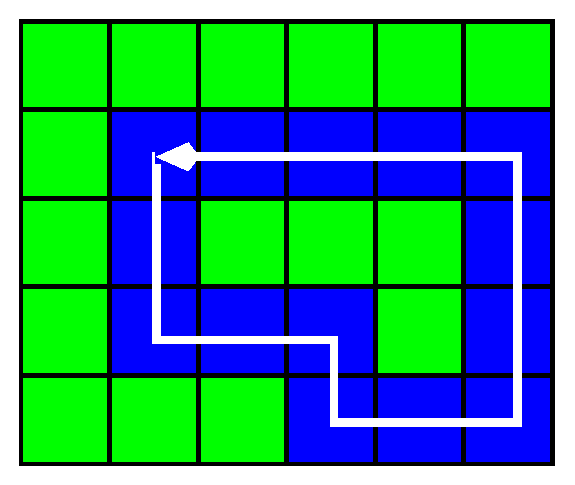
\psfig{file=img/race_track_flat.eps,width=5cm}}
\subfigure[Augmented dynamics]{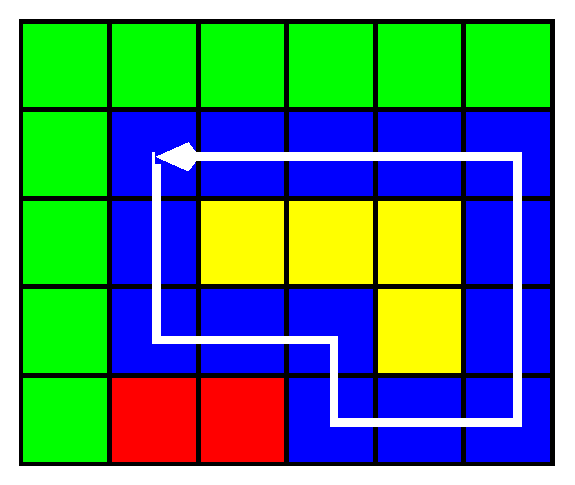
\psfig{file=img/race_track.eps,width=5cm}}\\}
\caption{\label{race_path}Unmodified (passive) and augmented environment dynamics for race path finding (colours naturally encode traversability of the cell)}
\end{figure*}

\end{document}
